\chapter{研究方案}

\section{建模}
采用形式化建模语言、安全策略与应用软件的模型融合等关键技术对应用软件进行建模。由于应用软件具有分布性、异构性、并发性和实时性等特征,采用拓扑图和状态机相结合的方式可以准确描述应用软件的上述性质。
\par
\begin{figure}[h]
	\centering
	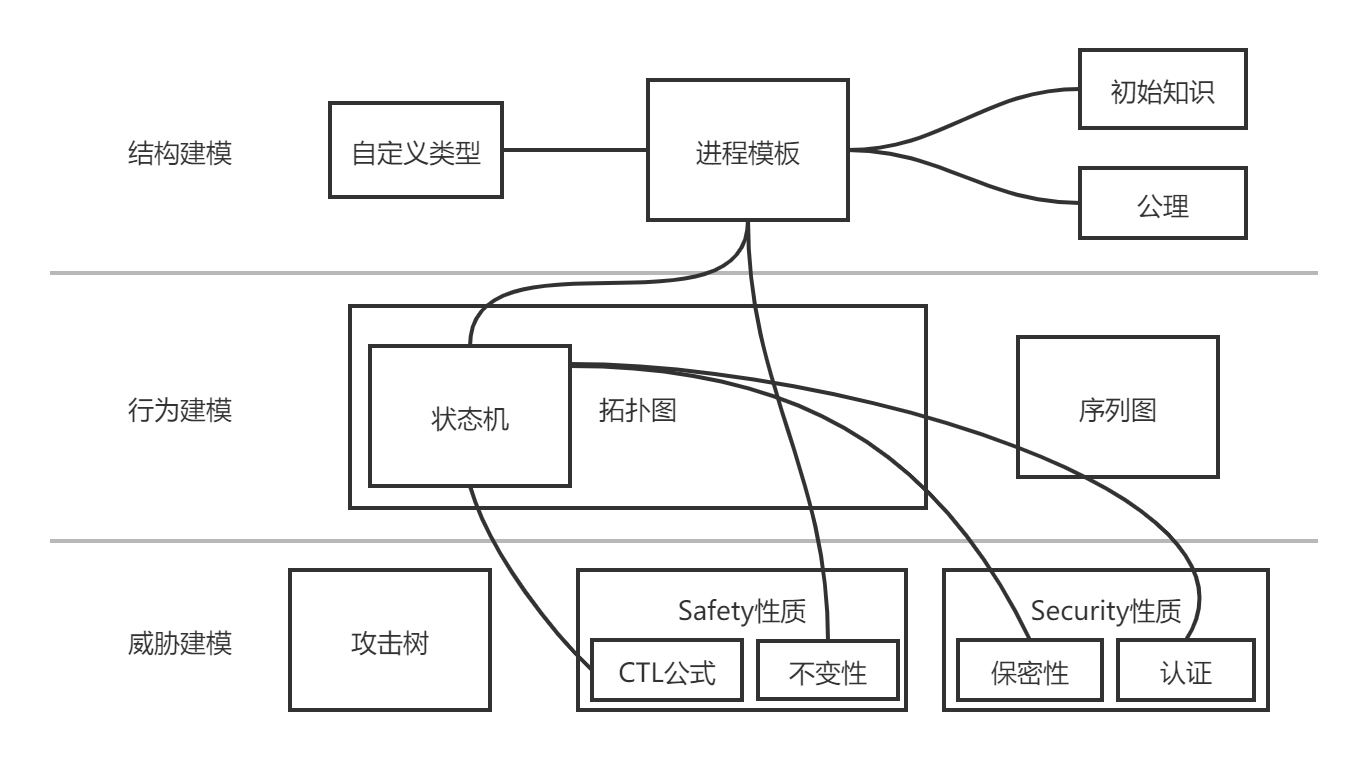
\includegraphics[width=12cm,height=6.75cm]{imgs/architecture.png}
	\caption{整体架构图}
	\label{architecture}
\end{figure}
\par
应用软件具有分布式特性,一般包括多个计算节点,单个节点进行实时计算,而节点之间通过异步消息传递来通信,因此对于分布性而言,是基于拓扑图的各个结点可以表达应用软件的不同行为。
\par
而对于异构性而言,是基于用户可以灵活架设拓扑图的二维拓扑结构;对于并发性而言,是基于拓扑图在拓扑排序上存在同层的行为结点;对于实时性而言,则要依靠拓扑图和状态机相结合的方式保证。
\par
以下将分别阐述用户建模过程中涉及的各类模型。

\subsection{类图建模}
类图定义了模型的静态结构,特别是模型中存在的类、类的内部结构以及它们与其他类的关系等,它是面向对象建模的重要组成部分。使用类图来对系统中涉及的各个数据结构进行建模。如网络协议中的消息包结构可使用类型嵌套的类图建模,协议的运作进程模板也将涉及程序初始变量和方法、通信方法等,同样使用相应的类图进行建模,其成分如图\ref{process}所示。
\begin{table}[h]
	\centering
	\begin{tabular}{|c|c|}
		\hline
		\textbf{成分} & \textbf{描述} \\ \hline
		Attribute           & 属性          \\ \hline
		Method              & 方法          \\ \hline
		CommMethod          & 通信手段        \\ \hline
	\end{tabular}
	\caption{进程模板类图中的成分}
	\label{process}
\end{table}

在对软件的进程模板进行建模时,还涉及进程模板的初始知识,即软件进程模板的哪些属性是软件运行初期就已知的,它也是使用类图进行建模。另外还涉及一些系统中复杂的先验知识,例如在协议中涉及到加密解密操作时,需要指明配对的加解密方法,这可以通过公理公式描述,也是使用类图进行建模。

\subsection{状态机建模}
状态机适合对分布式应用软件的单个节点的控制计算逻辑进行描述,在状态机的转移边上有转移条件和转移时执行的控制动作,整个状态机从初始状态到终止状态运行一遍,也就描述了软件进程从启动到结束的整个生命周期执行的行为,因此状态机建模是基于类图中进程模板的建模的。在我们的方案中,一个进程模板对应于一个状态机。同样地,对集中式的软件状态机仍然能够胜任行为建模。
\par
进程模板描述了软件对外可见的组成成分,而状态机描述了软件内部的行为,由于采用了统一语义框架的状态机和进程模板有机融合的建模语言,在状态机中可以使用进程模板暴露出的属性、方法和通信手段。以对软件执行过程中的细节进行描述。例如,网络安全协议中可以在某个状态向另一进程发送消息,而在另一状态等待消息接收并按照消息头来决定下一步的不同行为。
\par
需要注意的是,对分布式应用软件而言,将使用拓扑图描述整个软件系统。而状态机作为系统中单个结点的行为描述,也包括了分布式通信的行为,这也和进程模板本身的通信方法定义相关。总的来说,状态机在系统中将作为软件细节的重要描述手段,也是进程模板之间交互的建模中介。

\subsection{拓扑图建模}
拓扑图用于描述分布式软件的结点拓扑结构,对于每个结点而言,它可以选择使用已定义的进程模板,表示该结点所运行的进程。拓扑图中的不同结点可以使用不同的进程模板,也可以使用相同的进程模板,其意义即是从进程模板派生出各个具体的结点进程。
\par
由于进程模板使用唯一的状态机对其进程行为建模,所以软件的分布式结点将使用其行为作为结点的行为。但由于拓扑图中的结点还身处有向图中存在关系结构,所以其交互应具体受制于所处环境,这是拓扑图对分布式软件建模,特别是网络协议建模的重要作用。使用拓扑图用户可以构造网络中各个结点的拓扑结构,结合结点进程模板的状态机行为建模以实现对分布式网络协议的统一建模。

\subsection{序列图建模}
序列图是UML种的动态结构模型,用于描述执行系统功能的各个角色之间相互传递消息的顺序关系,显示对象之间的这些交互。序列图建模可以帮助用户理解和理清所建模的目标种存在哪些实体,以及他们之间的交互和信息传递顺序,也能帮助用户向其它用户传达系统流程和思想。
\par
在序列图中,主要涉及同步消息、异步消息和返回消息,其中同步消息和异步消息又可以分为到本对象的和到其它对象的。使用这样的方式可以帮助用户更好的描述系统流程中的同步和异步处理,并明确指出哪些消息是接收方对根据消息做出处理的响应,能够很好的适应网络协议建模。


\section{威胁和规约}
安全威胁模型是对整个攻击过程的结构化和系统化描述。开放式的网络环境以及分布式系统中应用软件的复杂特性使得对攻击模式描述越来越困难。拟研究能够对开放网络环境下应用软件多阶段安全威胁行为进行形式建模和分析的方法,研究安全策略(包括访问控制等)的形式建模方法。
\subsection{攻击树}
攻击树(Attack trees) 为我们提供了一种正式而条理清晰的方法来描述系统所面临的安全威胁和系统可能受到的多种攻击。我们用树型结构来表示系统面临的攻击,其中根节点代表被攻击的目标,叶节点表示达成攻击目标的方法。当攻击树应用在具体实例中时,其结构可能变得庞大而复杂。一个完整的攻击树很可能包括成百上千的叶节点,即便如此,攻击树也可以在很大程度上帮助我们判断系统存在的威胁和决定应对攻击的方法。本项目中攻击树的计算伪代码如下:
\lstset{
	caption=攻击树的计算, 
	basicstyle=\ttfamily\footnotesize,
	frame=tb,
	xleftmargin=.01\textwidth, xrightmargin=.01\textwidth
}
\begin{lstlisting}
def calculate(root):
	ans = false
	if (root.isActive):
		return calculate(root.childNodes[0])
	else:
		if root.condition == "ACTIVE":
			return calculate(root.childNodes[0])
		elif root.condition == "TRUE":
			return true
		elif root.condition == "FALSE":
			return false
		else:
			if root.name == "AND":
				ans = true
				for node in root.childNodes:
					if (!calculate(node)):
						ans = false
				return ans
			if root.name == "OR":
				ans = false
				for node in root.childNodes:
					if (calculate(node))
						ans = true
				return ans
			if root.name == "NEG":
				return !calculate(root.childNodes[0])

\end{lstlisting}
